\section{Design}

\subsection{Database}
The database is used to store all data regarding batches. Based on the
Enhanced Entity-Relationship Diagram (EER) in Figure \ref{figure:eer_diagram}
the SQL files can be written.

\begin{figure}[ht]
\centering 
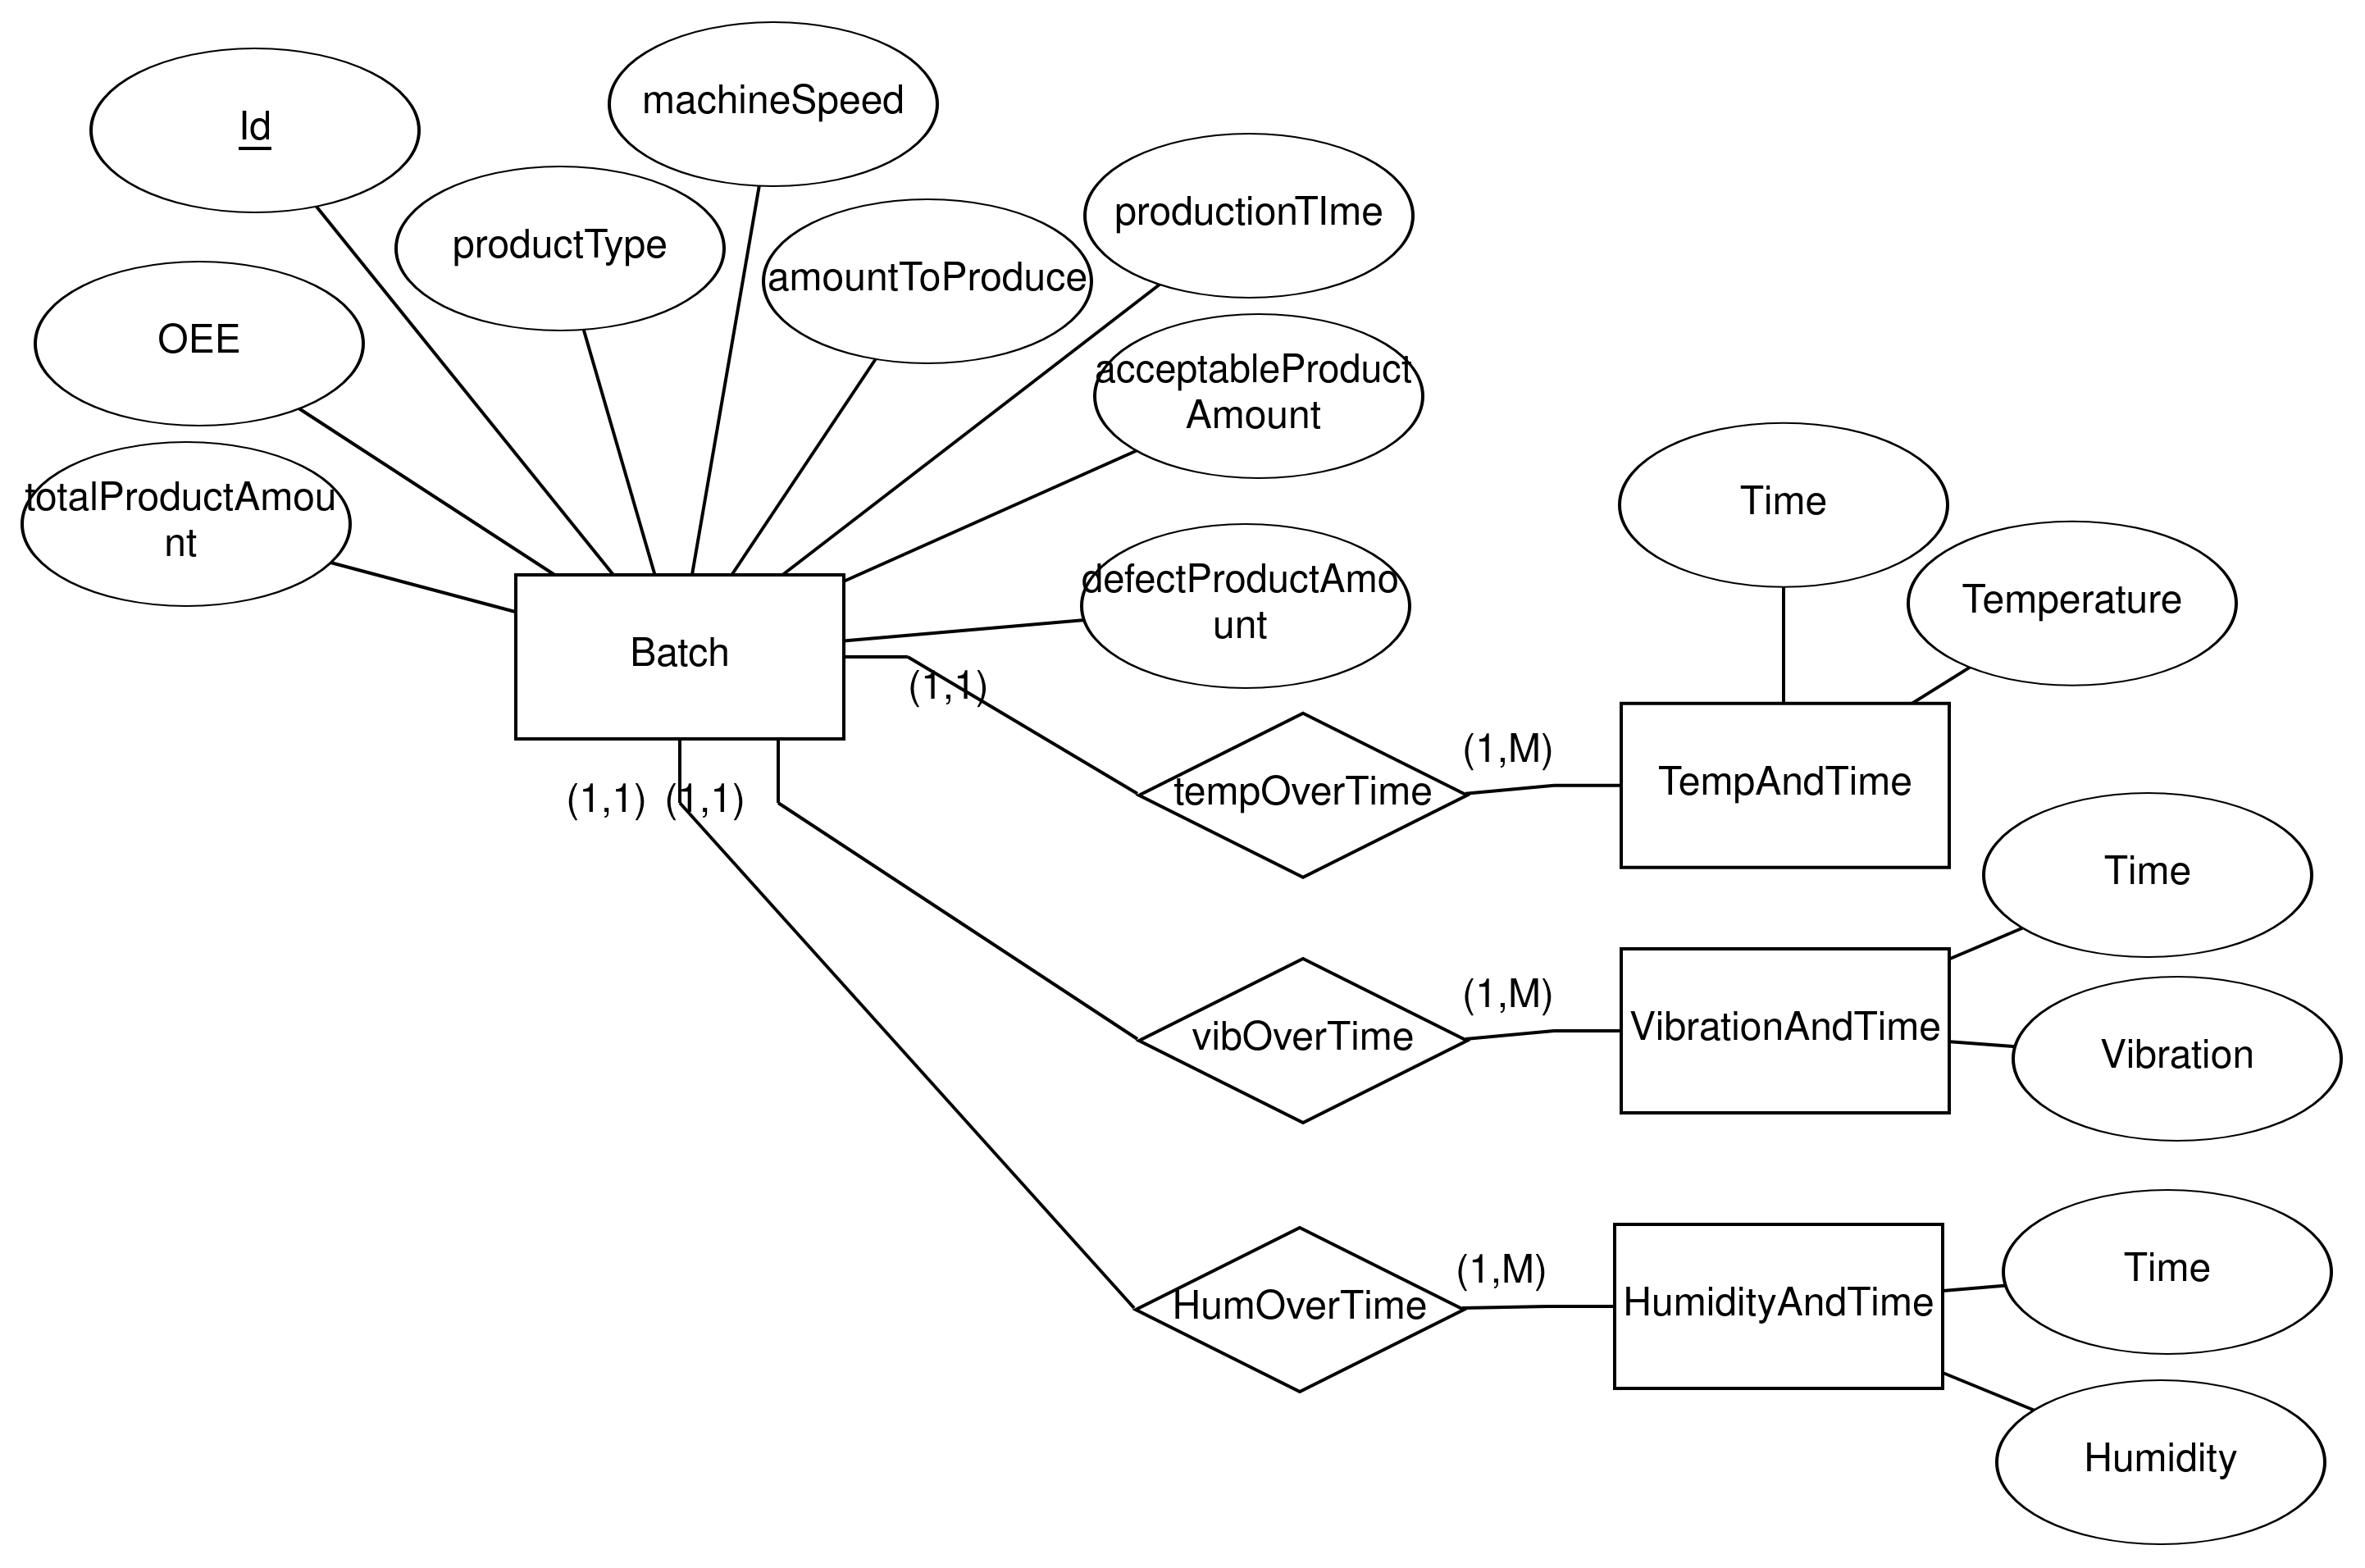
\includegraphics[width=0.8\linewidth]{images/eer_diagrams/database_EER_batch.png}
\caption{EER Diagram} 
\label{figure:eer_diagram}
\end{figure}

The database will have 4 main tables; batches, TempAndTime, VibrationAndTime and
HumidityAndTime. The batches table consists of all the data related to a
specific batch, such as id, product\_type, amount\_to\_produce, etc. The three
other tables will contain a timevalue and related data (temperature, vibration
and humidity).
Connecting the three tables to the batches table, are "subscription tables".
These will link a batch to temperature, vibration and humidity respectively,
using the ids.

\subsection{Dashboard}
A very important aspect the group has had to consider, is which design pattern
to model the dashboard after. A design pattern is a form of template, which in
this case, dictates how the different classes communicate. A relevant design
pattern is the MVC (Model - View - Controller). This pattern separates the
data-related logic (model), the UI logic (View) and the business logic 
(controller) into different layers, and thereby helps keep separation of
concerns. The controller manages input from the user, and forwards it to either
the model, to retrieve or store data, or the view, to present data to the user.\\

The group has decided to use the MVC design pattern, thus making it possible to
work on the different aspects of the system (GUI, database, logic) separately. 
A visualisation of the MVC pattern can be seen in figure \ref{figure:MVC_model}

\begin{figure}[H]
    \centering
    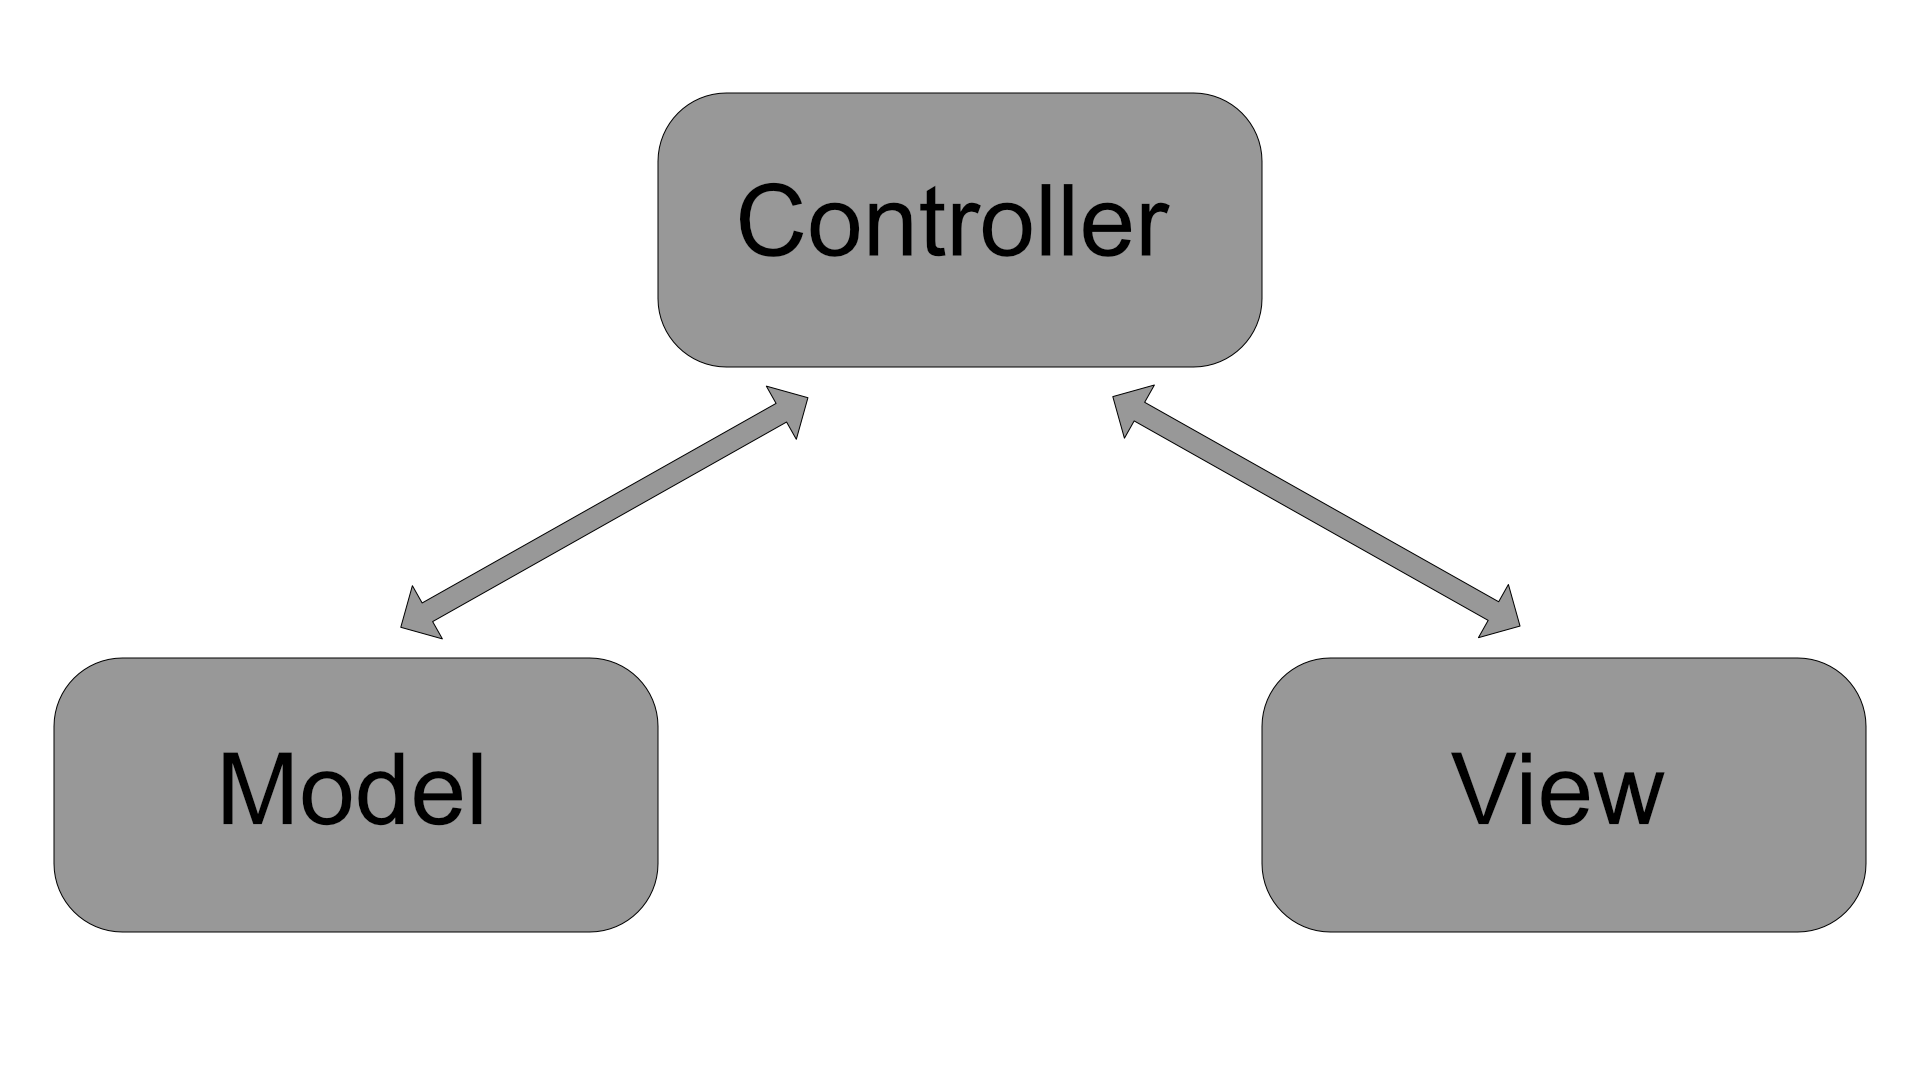
\includegraphics[scale=0.15]{images/MVC_model.png}
    \caption{MVC model}
    \label{figure:MVC_model}
\end{figure}

\subsection{OPC-UA Client}
The group was in doubt about the system being a monolith application containing 
the REST-API and OPC-UA Client in one program or split into two programs.

Choosing to split the program into two separate entities aligns with the 
separation of concerns principle ex. implementing authentication at a later 
stage(in the API) wouldn't affect the core logic of the OPC-UA client. On the 
other hand choosing to do so would add some overhead at the start of the 
implementation phase. \\

Another thing to consider when splitting the application into two separate 
entities is how they should interface with each other. To accomplish this the 
group has two options: 

\begin{table}[ht]
    \captionof{table}{Options}
    \begin{tabularx}{\textwidth}{|>{\RaggedRight}X|>{\RaggedRight}X|>{\RaggedRight}X|}
        \hline
        \textbf{Option} & \textbf{Pros} & \textbf{Cons} \\
        \hline
        Console Application & Simplest to implement & Connection to the OPC-UA 
        server is created for each request (Performance overhead)\\
        \hline
        HTTP server & Connection to OPC-UA server is made once and reused. HTTP
        naturally talks JSON which is ideal as an interface & Takes longer to 
        implement \\
        \hline
    \end{tabularx}
    \label{someLabel}
\end{table}

The group evaluated that the split up benefits outweighed the negatives. This 
decision demands that the client uses HTTP communication to communicate with the
API over localhost. 
